\chapter{Introduction}
\label{chap:chap1}

Nuclear-polarized noble gases have been proven to be very useful in various applications, such as polarized targets for electron scattering experiments~\cite{PhysRevLett.71.959}, magnetic resonance imaging~\cite{MRI} and neutron scattering experiments~\cite{Neutron}. Polarized $^3$He has been particularly useful for studying spin-dependent interactions involving neutrons because, to first-order approximation, a $^{3}$He nucleus has a pair of protons with paired spins and a single neutron that carries the most of the nuclear spin. Free neutrons are not used as targets because they decay with a lifetime of about 14 minutes, 42 seconds. 

\section{Overview of Recent Target Development}

An early use of polarized $^3$He target in electron scattering experiment was at Stanford Linear Accelerator Center (SLAC) in the year of 1992. The experiment was known as E142 and investigated the spin structure of neutrons~\cite{PhysRevLett.71.959}. Recent experiments were conducted at Jefferson Laboratory (JLAB) in Newport News, Virginia, such as ``Measurement of the Neutron Electric Form Factor $G^n_E$ at High $Q^2$", also known as E02-013~\cite{PhysRevLett.105.262302}. E06-10, E06-014 and E05-015 were experiments that investigated single-spin asymmetries~\cite{Coulter}. 

The $^3$He targets used in these experiments were polarized with the technique Spin-Exchange Optical Pumping (SEOP). Fig.~\ref{TargetCell} shows what a typical target looks like, they are also referred to as ``cells" very often. These cells were made of the GE180 glass and use a two-chambered design. The top chamber, known as the “pumping chamber”, is where $^{3}$He is polarized through SEOP. The bottom chamber, known as the “target chamber”, is where electron scattering occurs. The two ends of the target chamber where electron beam enters and exits are known as the ``end windows". Great effort has been made in our lab to develop this generation of cells. Alkali-hybrid SEOP together with narrowband laser diode arrays have increased the $^{3}$He polarization from 37\% to 70\%. Among other things, we also carefully studied an additional spin relaxation mechanism that limits the maximum achievable $^{3}$He polarization, which is referred to as the ``X Factor". Analysis of data accumulated through developing this generation of target cells were thoroughly discussed in Ref.~\cite{PhysRevC.91.055205}, part of which will be presented in chapter 4. 

\begin{figure}[H]
	\centering
	\resizebox{0.91\textwidth}{!}{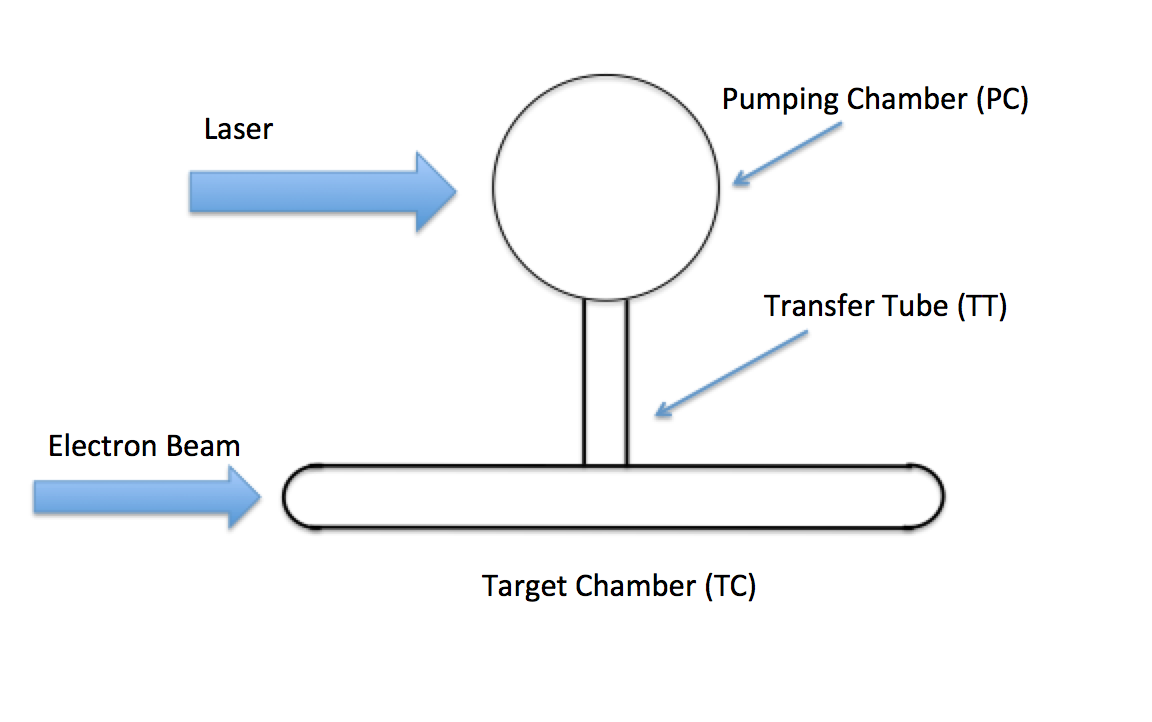
\includegraphics{TargetCell.png}}
	\caption{{ A schematic representation of a target cell. The dimensions of different parts of the cell are not to scale.}}
	\label{TargetCell}
\end{figure}

\section{New Generation Target Cells}

The future experiments planned during the 12GeV era after the upgrade will be much more demanding in terms of target cell performance. In particular, there is a desire to run experiments with higher luminosity where luminosity is the product of gas density in the target, interaction length and beam current. Increased luminosity will to more interactions that depolarize the target. We have designed and tested a new style cell that utilizes convection instead of diffusion to increase the rate at which the polarization in the target chamber is replenished by polarized gas from pumping chamber~\cite{PhysRevC.84.065201}. We have obtained over 50\% polarization with controllable convection speed so far.

An additional problem that comes with higher beam current is that the glass end windows of traditional design are not likely to survive the experiments. Our group started exploring the option of using metal end windows since eight years ago. Fig~\ref{metal_end_windows} shows an example configuration of such a target. The first problem to solve is to find out the correct material and the proper technique to incorporate metal without introducing significant spin relaxation and still being able to hold high pressure gas (12 atm) inside. This is a brand new technique that may have a profound impact on future cell designs once fully developed. Although no metal end windows have been tested so far, through carefully examining multiple glass cells with different kinds metal tubes (much larger in area compared to the end windows that will be used in JLAB experiments) attached, we have developed a reliable way of incorporating metal to target cells without introducing significant spin relaxation rates. We believe the next generation target cells used in the 12GeV era will be able to utilize metal end windows. In these test cells, the metals tubes were connected to Pyrex glass with Houskeeper seals~\cite{Houskeeper} and stayed intact through high pressure tests. After exploring options such as pure copper, gold coated copper, titanium, stainless steel, gold coated titanium, we have established that electroplating gold on copper substrate yields the best result so far, we have achieved a 15.6 h relaxation time with a Pyrex cell that had a 5'' long by 1'' gold coated copper tube attached horizontally. The additional relaxation rate introduced by the metal surface is proportional to the area of the gold surface. By comparing relaxation rate of test metal cells with pure-glass control cells, the relaxation rate due to gold surface was extrapolated. With this result, we believe the relaxation rate introduced by small metal windows in a target will be less than 1/135 hr$^{-1}$. To the best of our knowledge, our group was the first to have proved the potential of incorporating metal to target cells in the presence of alkali vapor. 

\begin{figure}[t!]\label{metal_end_windows}
	\centering
	\resizebox{0.91\textwidth}{!}{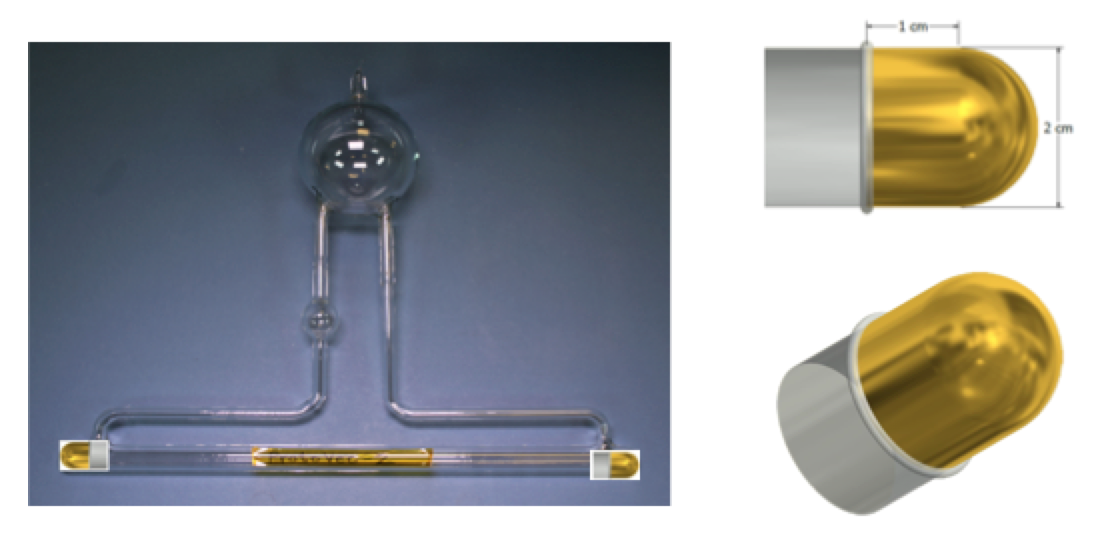
\includegraphics{metal_end_windows.png}}
	\caption{{A diagram of convection style target cell with metal end windows. }}
\end{figure}

\section{Structure of This Thesis}

This thesis focuses on both discussion on the development of high-performance polarized $3$He targets that utilize spin-exchange optical pumping (SEOP) and the development of future target cells that incorporate metal end windows. Chapter 2 gives a general description of SEOP. Chapter 3 introduces polarimetry techniques used in our lab for target cell characterization. Chapter 4 discusses the result collected in our lab from the over-a-decade development of $^3$He target cells, in which the spin-exchange rate constant for K and $^3$He is calculated and the so-called ``X Factor" is studied. Chapter 5 presents the development process of target cells with metal parts that aims to incorporate metal end windows to future cells for the 12 GeV era experiments. Chapter 6 summarizes this thesis and suggests future directions.













